\cleardoublepage

\chapter{Aplicación desarrollada}
\label{makereference5}

En este capítulo se introducirá la aplicación que se ha desarrollado con el
fin de demostrar los conceptos expuestos en los capítulos anteriores. En
concreto se desarrollarán shaders para los siguientes problemas:

\begin{itemize}
		\item Coloreado de terrenos
		\item Curvas de Bézier
		\item Superficies de Bézier
		\item Sólidos de revolución
		\item Nubes de puntos
		\item Negativo de una imagen
		\item Detección de bordes en una imagen
		\item Line Integral Convolution
\end{itemize}

Para el desarrollo de la aplicación y los shaders será necesario introducir
algunos conceptos matemáticos importantes, que se explican en la
sección~\ref{makereference5.1}.

\section{Plan de desarrollo}
\label{makereference5.1}

Durante las primera semanas de desarrollo de la aplicación lo más importante fue
realizar un exhaustivo estudio del funcionamiento de OpenGL, así como la lectura
y realización de tutoriales sobre la materia. Una vez adquirido el conocimiento
necesario, se comenzó a desarrollar el esqueleto principal de la aplicación,
sobre el cual se incorporarían después los distintos tipos de visualización a
realizar.\\

Una vez desarrollado este esqueleto se comenzó a la preparación de los shaders
que se utilizarían en cada uno de los problemas, para lo que se utilizó en gran
medida la información expuesta en el texto~\citet{Bailey}.\\

El siguiente paso fue conseguir datos y prepararlos adecuadamente para poder
mostrar las capacidades de visualización de la aplicación, así como comprobar su
correcto funcionamiento.\\

Lo anterior fue reiterado con cada uno de los problemas, añadiéndose cada vez
más a lo largo del desarrollo de todo el proyecto.

\section{Herramientas de desarrollo}
\label{makereference5.2}

Como entorno de desarrollo principal se ha utilizado el sistema operativo Ubuntu
Linux 18.04 LTS~\cite{UBUNTU}. En este sistema, además, se han utilizado las
siguientes herramientas de desarrollo:

\begin{itemize}
		\item Vim como editor de textos.~\cite{VIM}
		\item Git para el control de versiones.~\cite{GIT}
		\item Github como respositorio.~\cite{GITHUB}
		\item GCC como compilador.~\cite{GCC}
		\item GDB para la depuración.~\cite{GDB}
		\item Make para la gestión de dependencias.~\cite{MAKE}
\end{itemize}. 

Asimismo, siguiendo las recomendaciones del tutorial~\citet{LearnOpenGL}, se han
utilizado las siguientes librerías:

\begin{itemize}
		\item GLFW~\cite{GLFW}. GLFW es una librería orientada específicamente a
				OpenGL que proporciona las necesidades básicas para el
				renderizado en pantalla. Permite crear un contexto de OpenGL,
				definir parámetros de ventana y manejar la entrada del usuario.
				Estas son las funciones que utilizaremos en la aplicación.
		\item GLAD~\cite{GLAD}. La localización de funciones de OpenGL depende
				tanto del controlador gráfico utilizado como del sistema
				operativo utilizado. Esta localización es desconocida en tiempo
				de  compilación y ha de ser conseguida en tiempo de ejecución.
				Es, pues, tarea del programador conseguir la localización de
				estas funciones. GLAD es una  librería que realiza esta tarea
				automáticamente.
		\item Assimp~\cite{ASSIMP}. Assimp --- \textit{The
				Open-Asset-Importer-Lib} --- es una librería que permite
				importar diferentes formatos de modelos 3D de una manera
				uniforme. Será utilizado para cargar los modelos para el
				colorado de terrenos.
		\item GLM~\cite{GLM}. GLM --- OpenGL Mathematics --- es una librería
				para matemáticas en software gráfico en C++ basada en las
				especificaciones del lenguaje GLSL. Proporciona funciones
				diseñadas e implementadas con el mismo convenio de nombres y
				funcionalidades que GLSL. Proporciona capacidades como
				transformaciones de matrices, cuaterniones, empaquetado de
				datos, aleatoriedad, ruido\ldots
		\item Otras librerías especificas del sistema operativo, como Pthreads,
				xrandr, x11, xi, xcursor, etc.
\end{itemize}

\section{Diseño de la aplicación}
\label{makereference5.3}

Para esta aplicación se ha optado por un diseño modular orientado a objetos, en
el que poder incrementalmente añadir distintos tipos de visualización sin tener
demasiados problemas. Como se ha expuesto en la sección~\ref{makereference5.1}
la aplicación consta de un esqueleto principal utilizado por todos los tipos de
visualización. Este esqueleto consta de una ventana principal, creada en el
programa principal, en la que se renderizará el objeto particular que representa
el tipo de visualización. Así, con el fin de añadir un nuevo tipo de
visualización solo se habrían de realizar las siguientes acciones:

\begin{enumerate}
		\item Crear un nuevo objeto que implemente los métodos necesarios
				de la clase \verb|Object|.
		\item Añadir un nuevo modo al \verb|enum Modes|.
		\item Añadir las opciones necesarias para dicho objeto en el programa
				principal e incluir la nueva clase \verb|#include "class.h"|.
		\item Actualizar las dependencias en el Makefile.
\end{enumerate}

En esta ventana principal se tiene por defecto un sistema de cámara en primera
persona, con la capacidad de moverse para visualizar mejor detalles del objeto
en cuestión. Este sistema puede ser sobreescrito en el objeto específico en
caso de necesitar otro comportamiento. \\

En la clase \verb|Object| existen tres métodos virtuales puros, que han de ser
implementados por las clases específicas de cada tipo de visualización:

\begin{itemize}
		\item \verb|draw()|, que ha de encargarse de dibujar el objeto en
				cuestión.
		\item \verb|processInputGLFWwindow * window)|, que ha de especificar que
				hacer con la entrada del usuario para este tipo de
				visualización.
		\item \verb|setUniforms()|, que ha de especificar las variables
				\verb|uniform| que utilicen los shaders de este tipo de
				visualización.
\end{itemize}

Estos métodos se llaman una vez por vuelta del bucle principal. En la sección
siguiente se introducen las matemáticas necesarias e importantes para el
desarrollo de la aplicación y los shaders concretos.

\section{Matemáticas necesarias}
\label{makereference5.4}

Con el fin de desarrollar el sistema de cámaras que utiliza la aplicación es
necesario conocer varios conceptos importantes sobre álgebra, geometría lineal y
transformaciones matriciales, así como los ángulos de Euler y su relación con
los cuaterniones. También se explorarán distintos métodos numéricos, relevantes
en el método de Line Integral Convolution, así como fórmulas matemáticas
específicas de cada tipo de visualización.

\subsection{Transformaciones matriciales}
\label{makereference5.4.1}

Como vamos a trabajar con objetos tridimensionales y una cámara móvil,
necesitamos realizar transformaciones sobre los vértices que componen nuestros
objetos para que estos aparezcan en su lugar y con sus dimensiones adecuadas.
Es deseable, además, realizar estas operaciones con vectores matricialmente,
puesto que éstas permiten presentar transformaciones arbitrarias en un
formato consistente y apto para la computación. Así, se pueden concatenar
diferentes transformaciones de manera sencilla multiplicando sus matrices. \\

Entre estas transformaciones podemos encontrar lineales y no lineales. Así, para
representar matricialmente transformaciones no lineales en un espacio Euclídeo
$n$-dimensional $\mathbb{R}^n$ se puede utilizar una transformación lineal en el
espacio $(n+1)$-dimensional $\mathbb{R}^{n+1}$. Este tipo de transformaciones
incluye tanto las transformaciones afines (como la
traslación~\ref{makereference5.4.1.1}) como transformaciones proyectivas.\\

Esta es la razón por la que las matrices $4 \times 4$ son tan ampliamente
utilizadas en la informática gráfica y, en consecuencia, en nuestra
aplicación.\\

En esta sección se presentan las transformaciones lineales y afines más
habituales y necesarias para nuestra aplicación, así como sus formas
matriciales. \\

\subsubsection{Traslación}
\label{makereference5.4.1.1}

Se denomina traslación a la operación consistente en \textit{mover} un vector en
una posición a otra nueva posición. Supongamos, pues, que queremos trasladar un
vector $\overrightarrow{v} = (x,y,z)$ en la dirección marcada por el vector
$\overrightarrow{t} = (t_1, t_2, t_3)$ como se muestra en la
figura~\ref{fig:translation}. Para ello realizaríamos la siguiente operación:\\

\begin{equation}
	\label{eq:translation}
	\overrightarrow{v}' = \overrightarrow{v} + \overrightarrow{t} = 
	\left( \begin{array}{c}
			x + t_1 \\
			y + t_2 \\
			z + t_3 \\
	\end{array} \right)
\end{equation}\\

La traslación se trata de una transformación afín sin puntos fijos. Como se ha
expuesto previamente, para poder representar esta transformación de forma
matricial se ha de recurrir a un espacio de una dimensión más. Por tanto, se
recurre a las coordenadas homogéneas para representar la traslación de un
espacio vectorial con multiplicación de matrices. Escribiendo el vector
$\overrightarrow{v} = (x,y,z)$ utilizando una cuarta coordenada homogénea
$\overrightarrow{v} = (x,y,z,1)$. Esta operación se muestra
en~\eqref{eq:matrixtranslation}. \\

\begin{equation}
	\label{eq:matrixtranslation}
	\overrightarrow{v}' = 
	\left( \begin{array}{cccc}
			1 & 0 & 0 & t_1 \\
			0 & 1 & 0 & t_2 \\
			0 & 0 & 1 & t_3 \\
			0 & 0 & 0 & 1 \\
	\end{array} \right)
	\left( \begin{array}{c}
			x \\
			y \\
			z \\
			1 \\
	\end{array} \right) = 
	\left( \begin{array}{c}
			x + t_1 \\
			y + t_2 \\
			z + t_3 \\
			1 \\
	\end{array} \right)
\end{equation}\\

\subsubsection{Escalado}
\label{makereference5.4.1.2}

El escalado de un vector es la operación consistente en modificar la longitud
del vector. Para ello, debemos multiplicar cada una de sus coordenadas por el
factor de escalado deseado en cada eje. Es decir, para escalar un vector
$\overrightarrow{v}$ por un factor de $0.5$ en el eje $x$ y $3$ en el eje $y$,
la operación a realizar sería la siguiente:\\

\begin{equation}
	\label{eq:scaling}
	\overrightarrow{v} = 
	\left( \begin{array}{c}
			2 \\
			3 \\
	\end{array} \right)
	\;\;\;\;\;
	\overrightarrow{v}' =
	\left( \begin{array}{c}
		2\cdot0.5 \\
		3\cdot3 \\
	\end{array}	\right) =  
	\left( \begin{array}{c}
			1 \\
			9 \\
	\end{array} \right)
\end{equation}\\

\begin{figure}[h]
	\centering
	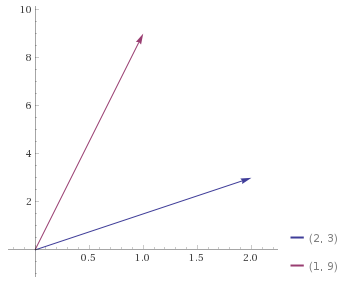
\includegraphics{figures/scaling.png}
	\caption{Escalar un vector}
	\label{fig:scaling}
\end{figure}

Esta operación de escalado se puede escribir matricialmente como sigue.
Supongamos que tenemos un vector $\overrightarrow{v}=(x,y,z)$ y lo queremos
escalar por un factor $fac=(F_1,F_2,F_3)$. Entonces podemos escribir la
operación anterior con la matriz $FAC$ como sigue:\\

\begin{equation}
	\label{eq:matrixscaling}
	\overrightarrow{v}' = 
	\left( \begin{array}{cccc}
			F_1 & 0   & 0   & 0	\\
			0   & F_2 & 0   & 0	\\
			0   & 0   & F_3 & 0	\\
			0   & 0   & 0   & 1	\\
	\end{array} \right)
	\left( \begin{array}{c}
			x \\
			y \\
			z \\
			1 \\
	\end{array} \right) =
	\left( \begin{array}{c}
			F_1\cdot x \\
			F_2\cdot y \\
			F_3\cdot z \\
			1 \\
	\end{array} \right)
\end{equation}\\

Nótese que también en este caso al vector $\overrightarrow{v}$ se le ha añadido
una cuarta coordenada $w$ con el fin de ser consistentes con aquellas
transformaciones no lineales que necesitan de un espacio de dimensión mayor. \\

\subsubsection{Rotación}
\label{makereference5.4.1.3}

Al contrario de los casos de la rotación y traslación de vectores expuestas
anteriormente, el caso de la rotación requiere un estudio más profundo en el
caso tridimensional para la matemática aplicada. Por esto, se dedica una sección
exclusiva para este tema. (Ver sección~\ref{makereference5.4.2}).

\subsection{Rotación: Ángulos de Euler y Cuaterniones}
\label{makereference5.4.2}

%% TODO

\subsection{Métodos Numéricos para la resolución de Ecuaciones Diferenciales}
\label{makereference5.4.3}

Como ya se vio en la sección~\ref{ref:lic}, en el método del Line Integral Convolution
se ha de utilizar un método numérico para computar la línea de flujo. En esta
sección se analizan algunos de los métodos utilizados y propuestos tanto
por~\citet{osti_10185520} como por \citet{licthesis}. 

\subsubsection{Método de Euler}
\label{makereference5.4.3.1}
\subsubsection{Método de Euler de paso variable}
\label{makereference5.4.3.2}
\subsubsection{Métodos de Runge-Kutta}
\label{makereference5.4.3.3}

\subsection{Otras Fórmulas}
\label{makereference5.4.4}

Para el desarrollo de la aplicación también se han tenido que utilizar fórmulas
matemáticas que describen el comportamiento de las curvas y superficies de
Bézier, ya explicadas en la sección~\ref{ref:bezier}, así como las
fórmulas para la obtención de los valores de los pixeles de salida en el método
del Line Integral Convolution (Sección~\ref{ref:lic}).

\section{Shaders en la aplicación}
\label{makereference5.5}

En esta sección se presentan ya los shaders desarrollados para cada uno de los
tipos de visualización considerados en el proyecto, analizando los distintos
cálculos realizados y explorando las entradas y salidas de cada uno de ellos.

\subsection{Coloreado de terrenos}
\label{makereference5.5.1}
\subsection{Curvas de Bézier}
\label{makereference5.5.2}
\subsection{Superficies de Bézier}
\label{makereference5.5.3}
\subsection{Sólidos de revolución}
\label{makereference5.5.4}
\subsection{Nube de puntos}
\label{makereference5.5.5}
\subsection{Negativo de una imagen}
\label{makereference5.5.6}
\subsection{Detección de bordes}
\label{makereference5.5.7}
\subsection{Line Integral Convolution}
\label{makereference5.5.8}
